\documentclass{beamer}

\newcommand{\lesson}{Polymorphism}


\newcommand{\course}{Introduction to Object-Oriented Programming}
\subject{\course}
\title[\lesson]{\course}
\subtitle{\lesson}

\author[CS 1331]
{Christopher Simpkins \\\texttt{chris.simpkins@gatech.edu}}
\institute[Georgia Tech]

\date[]{}

\newcommand{\link}[2]{\href{#1}{\textcolor{blue}{\underline{#2}}}}
\newcommand{\code}{http://www.cs1331.org/code}

\usepackage{colortbl}

% If you have a file called "university-logo-filename.xxx", where xxx
% is a graphic format that can be processed by latex or pdflatex,
% resp., then you can add a logo as follows:

% \pgfdeclareimage[width=0.6in]{coc-logo}{cc_2012_logo}
% \logo{\pgfuseimage{coc-logo}}

\mode<presentation>
{
  \usetheme{Berlin}
  \useoutertheme{infolines}

  % or ...

 \setbeamercovered{transparent}
  % or whatever (possibly just delete it)
}

\usepackage{tikz}
% Optional PGF libraries
\usepackage{pgflibraryarrows}
\usepackage{pgflibrarysnakes}
\usepackage{pgfplots}
\usepackage{fancybox}
\usepackage{listings}
\usepackage{hyperref}
\hypersetup{colorlinks=true,urlcolor=blue}
\usepackage[english]{babel}
% or whatever

\usepackage[latin1]{inputenc}
% or whatever

\usepackage{times}
\usepackage[T1]{fontenc}
% Or whatever. Note that the encoding and the font should match. If T1
% does not look nice, try deleting the line with the fontenc.


\usepackage{listings}

% "define" Scala
\lstdefinelanguage{scala}{
  morekeywords={abstract,case,catch,class,def,%
    do,else,extends,false,final,finally,%
    for,if,implicit,import,match,mixin,%
    new,null,object,override,package,%
    private,protected,requires,return,sealed,%
    super,this,throw,trait,true,try,%
    type,val,var,while,with,yield},
  otherkeywords={=>,<-,<\%,<:,>:,\#,@},
  sensitive=true,
  morecomment=[l]{//},
  morecomment=[n]{/*}{*/},
  morestring=[b]",
  morestring=[b]',
  morestring=[b]""",
}

\usepackage{color}
\definecolor{dkgreen}{rgb}{0,0.6,0}
\definecolor{gray}{rgb}{0.5,0.5,0.5}
\definecolor{mauve}{rgb}{0.58,0,0.82}

% Default settings for code listings
\lstset{frame=tb,
  language=scala,
  aboveskip=2mm,
  belowskip=2mm,
  showstringspaces=false,
  columns=flexible,
  basicstyle={\scriptsize\ttfamily},
  numbers=none,
  numberstyle=\tiny\color{gray},
  keywordstyle=\color{blue},
  commentstyle=\color{dkgreen},
  stringstyle=\color{mauve},
  frame=single,
  breaklines=true,
  breakatwhitespace=true,
  keepspaces=true
  %tabsize=3
}


% \beamerdefaultoverlayspecification{<+->}


\begin{document}

\begin{frame}
  \titlepage
\end{frame}

%------------------------------------------------------------------------
\begin{frame}[fragile]{Introduction to Object-Oriented Programming}


Today we'll learn how to combine all the elements of object-oriented programming in the design of a program that handles a company payroll.  Object-oriented programming requires three features:
\begin{itemize}
\item Data abstraction with classes (encapsulation)
\item Inheritance
\item Dynamic method binding
\end{itemize}

That last part, dynamic method binding, provides for subtype {\it polymorphism}, which we'll learn today.

\end{frame}
%------------------------------------------------------------------------

%------------------------------------------------------------------------
\begin{frame}[fragile]{Class Hierarchies}

\vspace{-.05in}
Class hierarchies depict the superclass-subclass relationships between families of related classes.  Consider:
\vspace{-.05in}
\begin{center}
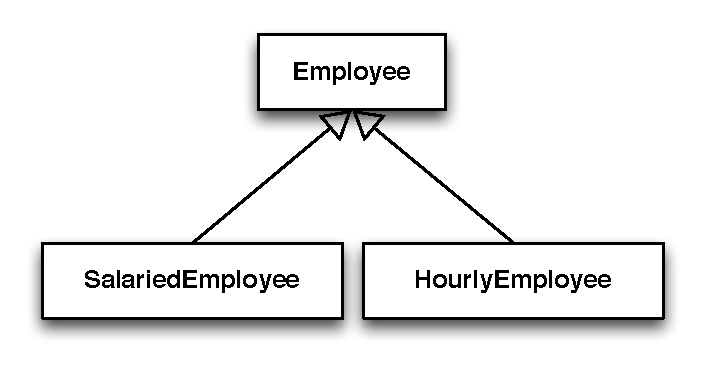
\includegraphics[height=1.4in]{employee-class-hierarchy.pdf}
\end{center}
\vspace{-.2in}
\begin{itemize}
\item {\tt Employee} is the superclass of {\tt HourlyEmployee} and {\tt SalariedEmployee}
\item {\tt Employee} is more general than {\tt HourlyEmployee} and {\tt SalariedEmployee}, e.g., there at least as many {\tt Employee}s as either {\tt HourlyEmployee}s or {\tt SalariedEmployee}s
\item {\tt HourlyEmployee} and {\tt SalariedEmployee} are richer than {\tt Employee} becuse they extend {\tt Employee} with additional features
\end{itemize}


\end{frame}
%------------------------------------------------------------------------

%------------------------------------------------------------------------
\begin{frame}[fragile]{A {\tt SalariedEmployee} Class}


Let's add {\tt SalariedEmployee} to our class hierarchy.  Here are the important pieces:
\begin{lstlisting}[language=Java]
public final class SalariedEmployee3 extends Employee3 {

    private static final int MONTHS_PER_YEAR = 12;
    private final double annualSalary;

    public SalariedEmployee3(String aName, Date aHireDate,
                            double anAnnualSalary) {
        super(aName, aHireDate);
        disallowZeroesAndNegatives(anAnnualSalary);
        annualSalary = anAnnualSalary;
    }
    public double getAnnualSalary() {
        return annualSalary;
    }
    public double monthlyPay() {
        return annualSalary / MONTHS_PER_YEAR;
    }
    // ...
}
\end{lstlisting}

\end{frame}
%------------------------------------------------------------------------

%------------------------------------------------------------------------
\begin{frame}[fragile]{Our {\tt Employee} Class Hierarchy}


We now have all the classes in our hierarchy:
\vspace{-.1in}
\begin{center}
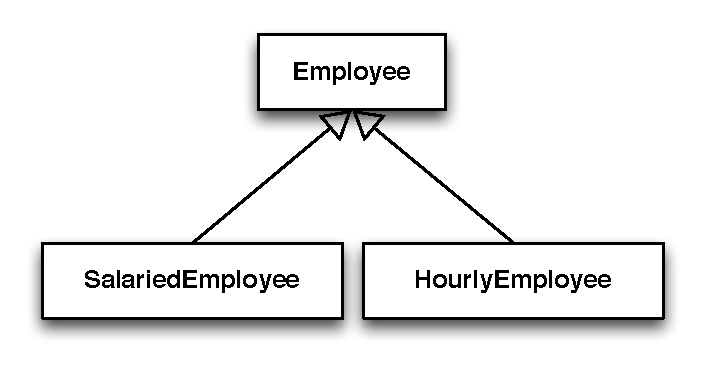
\includegraphics[height=1.1in]{employee-class-hierarchy.pdf}
\end{center}
\vspace{-.2in}
But our classes aren't well factored.
\begin{itemize}
\item {\tt SalariedEmployee3} and {\tt HourlyEmployee3} have duplicate copies of {\tt disallowZeroesAndNegatives}
\item {\tt SalariedEmployee3} and {\tt HourlyEmployee3} both have {\tt monthlyPay} methods, but these methods are not polymorphic because they're not defined in {\tt Employee3}
\end{itemize}

Let's refactor our {\tt Employee} class hierarchy to give it a clean object-oriented design.

\end{frame}
%------------------------------------------------------------------------

%------------------------------------------------------------------------
\begin{frame}[fragile]{A Company Spec}


Before we make {\tt monthlyPay} polymorphic, we need an application to demonstrate why doing so is useful.  Let's design a {\tt Company} class with the following specs:

\begin{itemize}
\item A {\tt Company4} has exactly 9 employees (becuase we haven't learned about dynamically resized data structures yet)
\item A company calculates its monthly payroll by adding up the monthly pay of each of its employees.
\item A company can have any mix of hourly and salaried employees
\end{itemize}

That last bullet motivates the use of polymorphism.

\end{frame}
%------------------------------------------------------------------------

%------------------------------------------------------------------------
\begin{frame}[fragile]{Maintaining an Employee List}


With our current class hierarchy, we need to maintain separate (partial) arrays of hourly and salaried employees.  Because they're partial arrays we also need to keep track of how many of each type of employee we have.
\begin{lstlisting}[language=Java]
public class Company {

    private HourlyEmployee[] hourlyEmployees;
    private int numHourlyEmployees = 10;
    private SalariedEmployee[] salariedEmployees;
    private int numSalariedEmployees = 10;

    public Company() {
        hourlyEmployees = new HourlyEmployee[numHourlyEmployees];
        salariedEmployees = new SalariedEmployee[numSalariedEmployees];
    }
}
\end{lstlisting}


\end{frame}
%------------------------------------------------------------------------

%------------------------------------------------------------------------
\begin{frame}[fragile]{Calculating Payroll the Hard Way}


With our employee lists, calculating payroll is accomplished with two loops:
\begin{lstlisting}[language=Java]
public class Company { // hypothetical

    public double monthlyPayroll() {
        double payroll = 0.0;
        for (int i = 0; i < numHourlyEmployees; ++i) {
            payroll += hourlyEmployees[i].monthlyPay();
        }
        for (int i = 0; i < numSalariedEmployees; ++i) {
            payroll += salariedEmployees[i].monthlyPay();
        }
        return payroll;
    }
    // ..
}
\end{lstlisting}
Seems reasonable.  But ...
\begin{itemize}
\item What if we want to add a third type of employee?
\end{itemize}


\end{frame}
%------------------------------------------------------------------------

%------------------------------------------------------------------------
\begin{frame}[fragile]{Calculating Payroll the Easy Way}


We'd like to be able to calculate payroll with a single loop over all employees:
\begin{lstlisting}[language=Java]
public class Company4 {

    public double monthlyPayroll() {
        double payroll = 0.0;
        for (Employee employee: employees) {
            payroll += employee.monthlyPay();
        }
        return payroll;
    }
    // ..
}
\end{lstlisting}

Much cleaner and less error-prone (e.g., we don't have the book-keeping of two partial arrays).  To be able to code like this we need to update the design of our {\tt Employee} class hierarchy.


\end{frame}
%------------------------------------------------------------------------

%------------------------------------------------------------------------
\begin{frame}[fragile]{A More General Employee List}

\vspace{-.05in}
The first step is to store one array of {\tt Employee}s:
\vspace{-.05in}
\begin{lstlisting}[language=Java]
public class Company4 {
    private Employee4[] employees;
    public Company4() {
        employees = ...;
    }
    public double monthlyPayroll() {
        double payroll = 0.0;
        for (int i = 0; i < employees.length; ++i) {
            payroll += employees[i].monthlyPay();
        }
        return payroll;
    }
}
\end{lstlisting}
\vspace{-.05in}
Much better.  But it doesn't compile.  Why?
\vspace{-.05in}
\begin{lstlisting}[language=Java]
$ javac Company.java
Company.java:15: cannot find symbol
symbol  : method monthlyPay()
location: class Employee
            payroll += employees[i].monthlyPay();
\end{lstlisting}
% $

\end{frame}
%------------------------------------------------------------------------


%------------------------------------------------------------------------
\begin{frame}[fragile]{Abstract Classes}


We need {\tt Employee} to declare a {\tt monthlyPay} method for subclasses to define.  Since we don't have a general definition for {\tt monthlyPay} suitable for {\tt Employee}, {\tt Employee} will need to be abstract.
\begin{lstlisting}[language=Java]
public abstract class Employee4 {
    // ...
    public abstract double monthlyPay();
}
\end{lstlisting}
An abstract class
\begin{itemize}
\item cannot be instantiated,
\item may contain zero or more abstract methods, and
\item subclasses must either provide an implementation for abstract methods, or be declared {\tt abstract} themselves.
\end{itemize}

This makes sense for our {\tt Employee4} class.  We don't ever want to instantiate {\tt Employee4} objects.  {\tt Employee4} simply defines the common aspects of all employees, with subclasses filling in the details.

\end{frame}
%------------------------------------------------------------------------

%------------------------------------------------------------------------
\begin{frame}[fragile]{The {\tt Employee4} Class Hierarchy}

\begin{center}
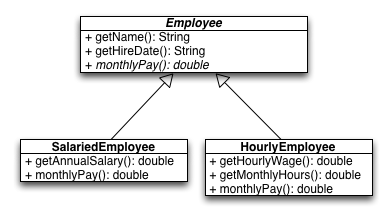
\includegraphics[height=1.5in]{employee-uml.png}
\end{center}
\begin{itemize}
\item {\tt Employee4} and its {\tt monthlyPay} method are abstract.
\item {\tt monthlyPay} is polymorphic because it is overriden in subclasses.
\end{itemize}
\end{frame}
%------------------------------------------------------------------------

%------------------------------------------------------------------------
\begin{frame}[fragile]{Polymorphic Methods}

\vspace{-.05in}
\begin{lstlisting}[language=Java]
public class Company4 {
    private Employee4[] employees;
    public double monthlyPayroll() {
        double payroll = 0.0;
        for (Employee4 employee: employees) {
            payroll += employees.monthlyPay();
        }
        return payroll;
    }
}
\end{lstlisting}
\vspace{-.1in}
\begin{itemize}
\item The static type of the elements of {\tt employees} is {\tt Employee4}
\item The dynamic type can be any subclass of {\tt Employee4}, in this case they are all {\tt SalariedEmployee4} and {\tt HourlyEmployee4}
\item When a method is invoked on an object, the method of the dynamic (run-time) type is used, no matter what the static (compile-time) type is.
\begin{itemize}
\item So though the static types of {\tt employees} elements is {\tt Employee}, the {\tt monthlyPay} methods invoked on them are the ones defined in {\tt SalariedEmployee4} and {\tt HourlyEmployee4}.
\end{itemize}
\end{itemize}
\end{frame}
%------------------------------------------------------------------------

%------------------------------------------------------------------------
\begin{frame}[fragile]{Refactoring Duplicate Code in a Class Hierarchy}

\vspace{-.05in}
Recall the definition of {\tt disallowZeroesAndNegatives}:
\vspace{-.05in}
\begin{lstlisting}[language=Java]
private void disallowZeroesAndNegatives(double ... args) {
    boolean shouldThrowException = false;
    String nonPositives = "";
    for (double arg: args) {
        if (arg <= 0.0) {
            shouldThrowException = true;
            nonPositives += arg + " ";
        }
    }
    if (shouldThrowException) {
        String msg = "Following arguments were <= 0: " + nonPositives;
        throw new IllegalArgumentException(msg);
    }
}
\end{lstlisting}
\vspace{-.075in}
\begin{itemize}
\item This method is duplicated in {\tt HourlyEmployee4} and {\tt SalariedEmployee4}
\item Let's move the definition of {\tt disallowZeroesAndNegatives} into {\tt Employee5} so it will be shared (rather than duplicated) in {\tt SalariedEmployee5} and {\tt HourlyEmployee5}.
\end{itemize}


\end{frame}
%------------------------------------------------------------------------

%% %------------------------------------------------------------------------
%% \begin{frame}[fragile]{Refactoring Common Code Into a Superclass}


%% After cutting {\tt disallowZeroesAndNegatives} from {\tt SalariedEmployee} and {\tt HourlyEmployee} and pasting it into {\tt Employee}, {\tt javac} tells us:
%% \begin{lstlisting}[language=Java]
%% $ javac Employee.java HourlyEmployee.java SalariedEmployee.java
%% HourlyEmployee.java:25: cannot find symbol
%% symbol  : method disallowZeroesAndNegatives(double,double)
%% location: class HourlyEmployee
%%         disallowZeroesAndNegatives(anHourlyWage, aMonthlyHours);
%%         ^
%% SalariedEmployee.java:17: cannot find symbol
%% symbol  : method disallowZeroesAndNegatives(double)
%% location: class SalariedEmployee
%%         disallowZeroesAndNegatives(anAnnualSalary);
%%         ^
%% 2 errors
%% \end{lstlisting}
%% % $

%% Why did we get these errors?

%% \end{frame}
%% %------------------------------------------------------------------------

%------------------------------------------------------------------------
\begin{frame}[fragile]{{\tt protected} Members}


{\tt private} members of a superclass are effectively invisible to subclasses.  To make a member accessible to subclasses, use {\tt protected}:
\begin{lstlisting}[language=Java]
public abstract class Employee5 {
    protected void disallowZeroesAndNegatives(double ... args) {
        // ...
    }
    // ...
}
\end{lstlisting}
{\tt protected} members
\begin{itemize}
\item are accessible to subclasses and other classes in the same package, and
\item can be overriden in subclasses.
\end{itemize}
{\tt protected} members provide encapsulation within a class hierarchy and package, {\tt private} provides encapsulation within a single class.\\
\vspace{.05in}
Later we'll see a better way to re-use.
\end{frame}
%------------------------------------------------------------------------

%------------------------------------------------------------------------
\begin{frame}[fragile]{The {\tt Employee} Class Hierarchy}

Let's add a summer intern class to our Employee hierarchy.
\vspace{-.1in}
\begin{center}
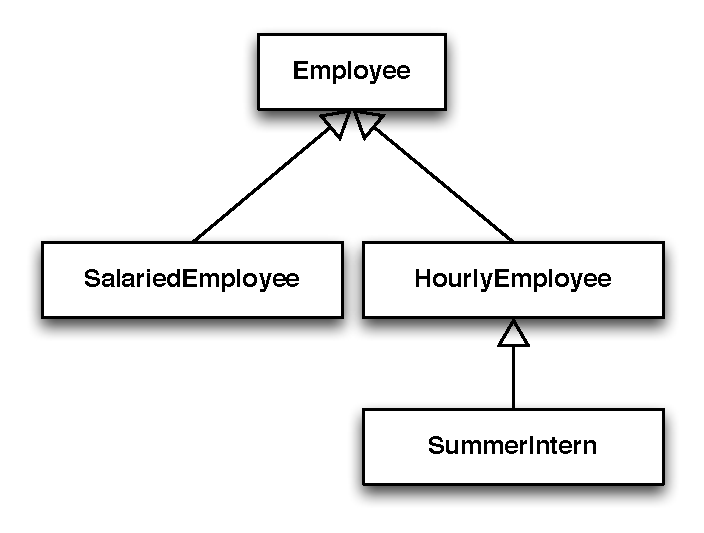
\includegraphics[height=1.5in]{expanded-employee-class-hierarchy.pdf}
\end{center}

\begin{itemize}
\item We can get the payRoll for the current month by making use of the polymorphic {\tt getMonthlyPay} method.
\item What if we wanted to get the payroll for a particular month?
\end{itemize}

Let's overload {\tt monthlyPay} so we can get the payroll for any month, not just the current month.

\end{frame}
%------------------------------------------------------------------------

%------------------------------------------------------------------------
\begin{frame}[fragile]{Enum Types}

Enums are data types that have a predefined set of constant values (\href{http://docs.oracle.com/javase/specs/jls/se7/html/jls-8.html#jls-8.9}{JLS \S 8.9}, \href{http://docs.oracle.com/javase/tutorial/java/javaOO/enum.html}{Java Enum Tutorial})

For example:
\begin{lstlisting}[language=Java]
public enum Month {
    JAN, FEB, MAR, APR, MAY, JUN, JUL, AUG, SEP, OCT, NOV, DEC
}
\end{lstlisting}
defines an enum type called {\tt Month} that can take on only one of the predefined constants {\tt Month.JAN}, {\tt Month.FEB}, ..., {\tt Month.DEC}

\begin{itemize}
\item Enum types are a class.
\item Java automatically defines convenience methods for enum types, like {\tt valueOf(String)} and {\tt values()} (See the \link{http://docs.oracle.com/javase/7/docs/api/java/lang/Enum.html}{Enum API}).
\item Because they define a class, enum types can include programmer-defined additional constructors and methods.
\end{itemize}

\end{frame}
%------------------------------------------------------------------------


%------------------------------------------------------------------------
\begin{frame}[fragile]{Ad-Hoc Polymorphism: Overloaded Methods}


An overloaded method is a set of methods with the same names but different signatures (parameter lists)\footnote{More precisely, two methods with the same name whose signatures are not {\it override-equivalent} are overloaded.} (\href{http://docs.oracle.com/javase/specs/jls/se7/html/jls-8.html#jls-8.4.9}{JLS \S 8.4.9}).\\
\vspace{.075in}
Here's an overloaded {\tt monthlyPay} for {\tt SummerIntern6}, along with a helper method demonstrating the use of the {\tt Month} enum:
\begin{lstlisting}[language=Java]
public double monthlyPay() {
    Date today = new Date();
    Month thisMonth = Month.values()[today.getMonth()];
    return monthlyPay(thisMonth);
}
public double monthlyPay(Month month) {
    return isSummer(month) ? super.monthlyPay() : 0.0;
}
private boolean isSummer(Month month) {
    return month == Month.JUN
        || month == Month.JUL
        || month == Month.AUG;
}
\end{lstlisting}
\vspace{-.075in}
\begin{itemize}
\item In which classes should these methods be declared? Defined?
\end{itemize}


\end{frame}
%------------------------------------------------------------------------

%------------------------------------------------------------------------
\begin{frame}[fragile]{The {\tt Employee} Class Hierarchy in UML}


\vspace{-.2in}
\begin{center}
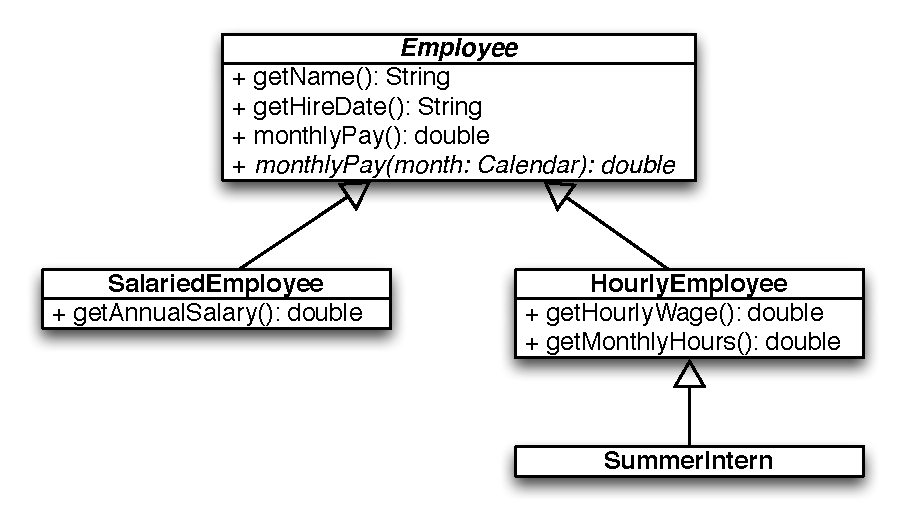
\includegraphics[height=1.5in]{employee-uml.pdf}
\end{center}
\vspace{-.25in}
\begin{itemize}
\item Italicized names are abstract (e.g., {\it Employee} is an abstract class, {\it + getMonthlyPay(month: Month)} is an abstract method).
\item We've only shown public methods (denoted by the '+' symbols in front of their names).
\item Each class has all the public methods in its superclasses, and possibly additional methods.
\item {\tt SummerIntern6} only {\it specializes} {\tt HourlyEmployee6}, that is, it modifies some behavior of its superclass but does not add any additional behavior.
\end{itemize}


\end{frame}
%------------------------------------------------------------------------

%------------------------------------------------------------------------
\begin{frame}[fragile]{Forecasting Payroll}


Now with our overloaded  {\tt montlyPay} method we can forecast payroll:
\begin{lstlisting}[language=Java]
  Company6 c = new Company6();
  System.out.println("Monthly payroll this month: " + c.monthlyPayroll());
  System.out.printf("Monthly payroll for May: %.2f%n",
                    c.monthlyPayroll(Month.MAY));
  System.out.printf("Monthly payroll for June: %.2f%n",
                    c.monthlyPayroll(Month.JUN));
\end{lstlisting}


\end{frame}
%------------------------------------------------------------------------

%------------------------------------------------------------------------
\begin{frame}[fragile]{Inheritance Hinders Re-use}

Recall the {\tt disallowZeroesAndNegatives} method that we refactored so that it's in the {\tt Employee} class and inherited by subclasses:
\vspace{-.05in}
\begin{lstlisting}[language=Java]
public abstract class Employee6 {
    protected void disallowZeroesAndNegatives(double ... args) {
        // ...
    }
}
\end{lstlisting}

\begin{itemize}
\item There's nothing about this method that is specific to {\tt Employee}s
\item {\tt disallowZeroesAndNegatives} could be useful in other classes that are not part of the {\tt Employee} class hierarchy.
\item Since it's {\tt protected}, it can't be used outside of the {\tt Employee} class hierarchy or package.
\end{itemize}

In software engineering terms, we say that the code in {\tt Employee} lacks {\it cohesion} - it has parts that aren't part of the {\it Employee} concept.  Such a design hinders reuse.

\end{frame}
%------------------------------------------------------------------------

%------------------------------------------------------------------------
\begin{frame}[fragile]{Favor Composition over Inheritance}

If we move these protected methods into a separate class, like \link{\code/employee/ValidationUtils.java}{ValidationUtils.java}
\begin{lstlisting}[language=Java]
public class ValidationUtils {

    public static void disallowNullArguments(Object ... args) { ... }

    public static void disallowZeroesAndNegatives(double ... args) { ... }
}
\end{lstlisting}
we can use them anywhere, e.g.,
\begin{lstlisting}[language=Java]
    public Employee(String aName, Date aHireDate) {
        ValidationUtils.disallowNullArguments(aName, aHireDate);
        name = aName;
        hireDate = aHireDate;
    }
\end{lstlisting}
With this refactoring, we have our final versions of \link{\code/employee/Employee.java}{Employee.java},
\link{\code/employee/HourlyEmployee.java}{HourlyEmployee.java}, and
\link{\code/employee/SalariedEmployee.java}{SalariedEmployee.java}

\end{frame}
%------------------------------------------------------------------------

%------------------------------------------------------------------------
\begin{frame}[fragile]{Closing Thoughts on Polymorphism}

We've now seen two kinds of polymorphism:
\begin{itemize}
\item Ad-hoc polymorphism (method overloading), and
\item Subtype polymorphism (overriding methods in subtypes).
\end{itemize}

{\it Subtype polymorphism} is core feature of OOP.  Polymorphism makes it possible to reuse {\it concepts} in a way that makes programs extensible without requiring rewriting existing code - this is the {\it open-closed principle}.\\
\vspace{.1in}
In the next block we'll see one more kind of polymorphism: type parameter polymorphism, or {\it parametric polymorphism}.
\end{frame}
%------------------------------------------------------------------------

%------------------------------------------------------------------------
\begin{frame}[fragile]{Object-oriented Design}

With encapsulation, inheritance, and polymorphism we have all the language features we need to employ three important object-oriented design principles:
\begin{itemize}
\item {\bf S}ingle responsiblity principle: a module should only contain code related to the definition of the module
  \begin{itemize}
    \item {\tt Employee} classes contain only employee-related code, validation code is in utility class
  \end{itemize}
\item {\bf O}pen-closed principle: open for extension, closed for modification
  \begin{itemize}
    \item Can add new {\tt Employee} subclasses without changing other classes in the {\tt Employee} hierarchy or classes that use {\tt Employee}s, such as {\tt Company}
  \end{itemize}
\item {\bf L}liskov substitution principle: instances of subtypes should be substitutable wherever instances of supertypes are expected
  \begin{itemize}
    \item A square is not a rectangle in an OO sense, but both are 2-D shapes
  \end{itemize}
\end{itemize}

In CS 2340 you'll learn several more OO design principles and several patterns that employ them.

\end{frame}
%------------------------------------------------------------------------


%% %------------------------------------------------------------------------
%% \begin{frame}[fragile]{Programming Exercise}


%% Expand on the {\tt Animal} and {\tt Dog} exercise by making the following changes:
%% \begin{itemize}
%% \item Make the {\tt speak} method in {\tt Animal} abstract.  What additional change to {\tt Animal} will you have to make?
%% \item Add a {\tt Cat} class which overrides {\tt speak} appropriately.
%% \item Create a {\tt Zoo} class that is just like {\tt Kennel} except that it
%%  maintains an array of {\tt Animal} (instead of {\tt Dog})
%% \end{itemize}


%% \end{frame}
%% %------------------------------------------------------------------------


% %------------------------------------------------------------------------
% \begin{frame}[fragile]{}


% \begin{lstlisting}[language=Java]

% \end{lstlisting}

% \begin{itemize}
% \item
% \end{itemize}


% \end{frame}
% %------------------------------------------------------------------------


\end{document}
